\subsection{AT Command Line Interface} 

A command-line interface (CLI) is a way to interact directly with the software of an embedded system in the form of text commands and responses. It can be seen as a typed set of commands to produce a result, but here, the commands are typed in real-time by a user through a specific interface, for example, UART, USB, LAN, etc. 

A CLI is often developed to aid initial driver development and debugging. This CLI might become the interface (or one of the interfaces) used by a sophisticated end-user to interact with the product. Think of typing commands to control a machine, or perhaps for low-level access to the control system as a development tool, tweaking time-constants and monitoring low-level system performance during testing. 

\subsubsection{The components of the CLI}
The provided development API parses and handles input commands, following a simplified form of the extended AT-commands syntax. 

\begin{figure}[H]
    \centering
    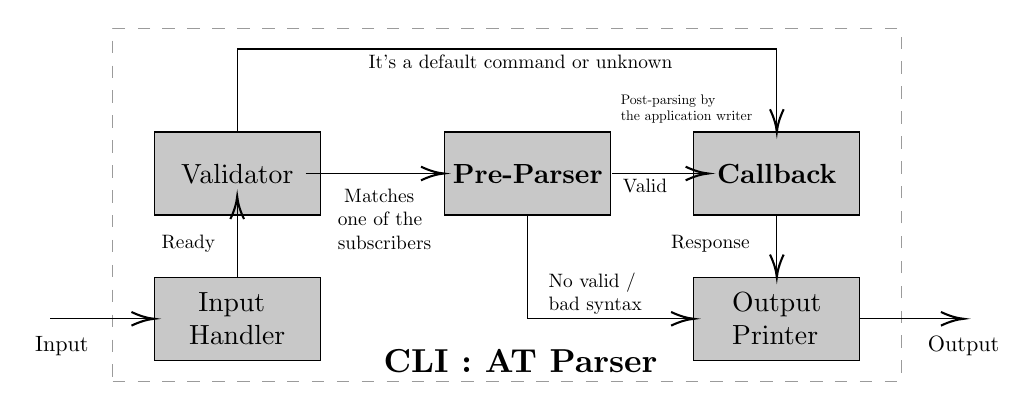
\begin{tikzpicture}[x=0.75pt,y=0.75pt,scale=1]
        \draw  [color={rgb, 255:red, 155; green, 155; blue, 155 }  ,draw opacity=1 ][fill={rgb, 255:red, 255; green, 255; blue, 255 }  ,fill opacity=1 ][dash pattern={on 4.5pt off 4.5pt}] (80,70) -- (460,70) -- (460,240) -- (80,240) -- cycle ;
        \draw  [fill={rgb, 255:red, 200; green, 200; blue, 200 }  ,fill opacity=1 ] (100,80) -- (180,80) -- (180,120) -- (100,120) -- cycle ;
        \draw  [fill={rgb, 255:red, 200; green, 200; blue, 200 }  ,fill opacity=1 ] (100,150) -- (180,150) -- (180,190) -- (100,190) -- cycle ;
        \draw  [fill={rgb, 255:red, 200; green, 200; blue, 200 }  ,fill opacity=1 ] (240,150) -- (320,150) -- (320,190) -- (240,190) -- cycle ;
        \draw  [fill={rgb, 255:red, 200; green, 200; blue, 200 }  ,fill opacity=1 ] (360,150) -- (440,150) -- (440,190) -- (360,190) -- cycle ;
        \draw  [fill={rgb, 255:red, 200; green, 200; blue, 200 }  ,fill opacity=1 ] (360,80) -- (440,80) -- (440,120) -- (360,120) -- cycle ;
        \draw    (140,190) -- (140,230) -- (400,230) -- (400,192) ;
        \draw [shift={(400,190)}, rotate = 450] [color={rgb, 255:red, 0; green, 0; blue, 0 }  ][line width=0.75]    (10.93,-3.29) .. controls (6.95,-1.4) and (3.31,-0.3) .. (0,0) .. controls (3.31,0.3) and (6.95,1.4) .. (10.93,3.29)   ;
        \draw    (50,100) -- (98,100) ;
        \draw [shift={(100,100)}, rotate = 180] [color={rgb, 255:red, 0; green, 0; blue, 0 }  ][line width=0.75]    (10.93,-3.29) .. controls (6.95,-1.4) and (3.31,-0.3) .. (0,0) .. controls (3.31,0.3) and (6.95,1.4) .. (10.93,3.29)   ;
        \draw    (440,100) -- (488,100) ;
        \draw [shift={(490,100)}, rotate = 180] [color={rgb, 255:red, 0; green, 0; blue, 0 }  ][line width=0.75]    (10.93,-3.29) .. controls (6.95,-1.4) and (3.31,-0.3) .. (0,0) .. controls (3.31,0.3) and (6.95,1.4) .. (10.93,3.29)   ;
        \draw    (400,150) -- (400,122) ;
        \draw [shift={(400,120)}, rotate = 450] [color={rgb, 255:red, 0; green, 0; blue, 0 }  ][line width=0.75]    (10.93,-3.29) .. controls (6.95,-1.4) and (3.31,-0.3) .. (0,0) .. controls (3.31,0.3) and (6.95,1.4) .. (10.93,3.29)   ;
        \draw    (280,150) -- (280,100) -- (358,100) ;
        \draw [shift={(360,100)}, rotate = 180] [color={rgb, 255:red, 0; green, 0; blue, 0 }  ][line width=0.75]    (10.93,-3.29) .. controls (6.95,-1.4) and (3.31,-0.3) .. (0,0) .. controls (3.31,0.3) and (6.95,1.4) .. (10.93,3.29)   ;
        \draw (400,170) node  [align=left] {\textbf{Callback}};
        \draw (280,170) node  [align=left] {\textbf{Pre-Parser}};
        \draw (140,170) node  [align=left] {Validator};
        \draw (400,100) node  [align=left] {Output\\Printer};
        \draw (140,100) node  [align=left] { \ Input\\Handler};
        \draw (55.5,87) node [scale=0.8] [align=left] {Input};
        \draw (490,87) node [scale=0.8] [align=left] {Output};
        \draw (368,136) node [scale=0.7] [align=left] {Response};
        \draw (336.5,164) node [scale=0.7] [align=left] {Valid};
        \draw (211,148) node [scale=0.7] [align=left] { \ Matches\\ one of the\\subscribers};
        \draw (276.5,224) node [scale=0.7] [align=left] {It's a default command or unknown};
        \draw (312.5,112) node [scale=0.7] [align=left] {No valid /\\bad syntax};
        \draw (356.5,201) node [scale=0.5] [align=left] {Post-parsing by \\the application writer};
        \draw (116.5,136) node [scale=0.7] [align=left] {Ready};
        \draw (276.5,79.5) node [scale=1.2] [align=left] {\textbf{CLI : AT Parser}};
        \draw    (173,170) -- (237.5,170) ;
        \draw [shift={(239.5,170)}, rotate = 180] [color={rgb, 255:red, 0; green, 0; blue, 0 }  ][line width=0.75]    (10.93,-3.29) .. controls (6.95,-1.4) and (3.31,-0.3) .. (0,0) .. controls (3.31,0.3) and (6.95,1.4) .. (10.93,3.29)   ;
        \draw    (320.5,170) -- (365,170) ;
        \draw [shift={(367,170)}, rotate = 180] [color={rgb, 255:red, 0; green, 0; blue, 0 }  ][line width=0.75]    (10.93,-3.29) .. controls (6.95,-1.4) and (3.31,-0.3) .. (0,0) .. controls (3.31,0.3) and (6.95,1.4) .. (10.93,3.29)   ;
        \draw    (140,120) -- (140,157) ;
        \draw [shift={(140,159)}, rotate = 270] [color={rgb, 255:red, 0; green, 0; blue, 0 }  ][line width=0.75]    (10.93,-3.29) .. controls (6.95,-1.4) and (3.31,-0.3) .. (0,0) .. controls (3.31,0.3) and (6.95,1.4) .. (10.93,3.29)   ;
    \end{tikzpicture}
    \caption{AT parser for a CLI implementation}
    \label{fig:atparser}
\end{figure}

As seen in figure \ref{fig:atparser}, the CLI has a few components described below:
\begin{itemize}
    \item  \textit{Input Handler} : It is responsible for collecting incoming data from the \textit{input} in the form of ASCII characters inside a buffer. When this buffer is ready by receiving an \lstinline{EOL}(\textit{End-Of-Line}) byte, it notifies the \textit{validator} to perform the initial checks.
    \item \textit{Validator}: Take the input string and perform three checks over it:
    \begin{enumerate}
        \item The input matches one of the subscribed commands.
        \item The input matches one of the default commands.
        \item The input is unknown
    \end{enumerate}
    \item \textit{Pre-Parser}: Takes the input if the \textit{validator} asserts the first check. It is responsible for syntax validation and classification. Also, prepares the input argument for the next component.
    \item \textit{Callback or Post-Parser}: If input at the \textit{pre-parser} is valid, the respective command-callback is invoked. Here, the application writer is free to handle the command execution and the output response.
    \item \textit{Output printer} : Takes all the return status of the previous components to print out a response at the output.
\end{itemize}
\bigskip

\begin{tcolorbox}
\HandRight Here, \textit{Input} and \textit{Output} should be provided by the application writer, for example, if a UART interface is chosen, the input should take the received bytes from an ISR and the output is a function to print out a single byte.
\end{tcolorbox}

\subsubsection{Supported syntax} \label{atsyntax}

The syntax is straightforward and the rules are provided below:

\begin{itemize}
    \item All command lines must start with \lstinline{AT} and end with an \lstinline{EOL} character. By default, the CLI uses the carriage return character. (We will use \lstinline{<CR>} to represent a carriage return character in this document).
    \item AT commands are case-insensitive 
    \item Only four types of AT commands are allowed:
    \begin{itemize}
        \item \textbf{Acting} (\lstinline{QATCLI_CMDTYPE_ACT}) : This is the simplest type of commands that can be subscribed. Its normally used to execute the action that the command should do. This type doesn't take arguments or modifiers, for example,
        \begin{lstlisting}
        AT+CMD
        \end{lstlisting}
        \item \textbf{Read} (\lstinline{QATCLI_CMDTYPE_READ}) : This type of command allows you to read or test a value already configured for the specified parameter. Only one argument is allowed.
        \begin{lstlisting}
        AT+CMD?
        AT+CMD?PARAM1
        \end{lstlisting}        
        \item \textbf{Test} (\lstinline{QATCLI_CMDTYPE_TEST}) : These types of commands allow you to get the values that can be set for its parameters. No parameters are allowed here.
        \begin{lstlisting}
        AT+CMD=?
        \end{lstlisting}
        \item \textbf{Parameter Set} (\lstinline{QATCLI_CMDTYPE_PARA}) : These types of commands allow \textit{n} arguments to be passed for setting parameters, for example:
        \begin{lstlisting}
        AT+CMD=x,y
        \end{lstlisting}
    \end{itemize}
    If none of the types is given at the input, the command response will be \lstinline{ERROR}
    \item The possible output responses are:
    \begin{itemize}
        \item \lstinline{OK}: Indicates the successful execution of the command.
        \item \lstinline{ERROR}: A generalized message to indicate failure in executing the command. 
        \item \lstinline{UNKNOWN} : The input command its not subscribed.
        \item \lstinline{NOT ALLOWED} : The command syntax is not one of the allowed types.
        \item \lstinline{User-defined}: A custom output message defined by the application writer.
        \item \lstinline{NONE} : No response.
    \end{itemize}
\end{itemize}

All responses are followed by a \lstinline{<CR><LF>}.
\medskip

Errors generated during the execution of these AT commands could be due to the following reasons:
\begin{itemize}
    \item Incorrect syntax/parameters of the AT command
    \item Bad parameters or not allowed operations defined by the application writer.
\end{itemize}

In case of an error, the string \lstinline{ERROR} or \lstinline{ERROR:<error_no>} are displayed.

\subsubsection{Setting up an AT-CLI instance}
Before starting the CLI development, the corresponding instance must be defined; a data structure of type \lstinline{qATCLI_t} \index{\lstinline{qATCLI_t}}. 
The instance should be initialized using the \lstinline{qATCLI_Setup()} API \index{\lstinline{qATCLI_Setup}}. A detailed description of this function is shown bellow:
\medskip

\begin{lstlisting}[style=CStyle]
qBool_t qATCLI_Setup( qATCLI_t * const cli, const qPutChar_t OutputFcn, 
                      char *Input, const size_t SizeInput, char *Output, 
                      const size_t SizeOutput, const char *Identifier, 
                      const char *OK_Response, const char *ERROR_Response, 
                      const char *NOTFOUND_Response, const char *term_EOL )
\end{lstlisting}

\subsubsection*{Parameters}
\begin{itemize}
    \item \lstinline{cli} : A pointer to the AT Command Line Interface instance. 
    \item \lstinline{OutputFcn} : The basic output-char wrapper function. All the CLI responses  will be printed-out through this function.
    \item \lstinline{Input} : A memory location to store the parser input (mandatory) 
    \item \lstinline{SizeInput} : The size of the memory allocated in \lstinline{Input}. 
    \item \lstinline{Output} : A memory location to store the parser output. If not used, pass \lstinline{NULL}.
    \item \lstinline{SizeOutput} : The size of the memory allocated in \lstinline{Output}. 
    \item \lstinline{Identifier} : The device identifier string. This string will be printed-out after a call to the \lstinline{AT_DEFAULT_ID_COMMAND}.
    \item \lstinline{OK_Response} : The output message when a command callback returns \lstinline{QATCLI_OK}. To use the default, pass \lstinline{NULL}.
    \item \lstinline{ERROR_Response} : The output message when a command callback returns \lstinline{QATCLI_ERROR} or any \lstinline{QATCLI_ERRORCODE(#)}. To use the default, pass \lstinline{NULL}.
    \item \lstinline{NOTFOUND_Response } : The output message when input doesn't match with any of  the available commands. To use the default, pass \lstinline{NULL}.
    \item \lstinline{term_EOL} : The \textit{End-Of-Line} string printed out after any of the parser messages. To use the default, pass \lstinline{NULL}. 
\end{itemize}

\subsubsection{Subscribing commands to the parser}
The AT CLI is able to subscribe any number of custom AT commands. For this, the 
\lstinline{qATCLI_CmdSubscribe()} \index{\lstinline{qATCLI_CmdSubscribe}} API should be used.

This function subscribes the CLI instance to a specific command with an associated callback function, so that next time the required command is sent to the CLI input, the callback function will be executed.
\medskip
The CLI module only analyzes commands that follow the simplified AT-Commands syntax already described in section \ref{atsyntax}.
\medskip

\begin{lstlisting}[style=CStyle]
qBool_t qATCLI_CmdSubscribe( qATCLI_t * const cli, 
                             qATCLI_Command_t * const Command, 
                             const char *TextCommand, 
                             qATCLI_CommandCallback_t Callback, 
                             qATCLI_Options_t CmdOpt, void *param )
\end{lstlisting}

\subsubsection*{Parameters}
\begin{itemize}
    \item \lstinline{cli} : A pointer to the AT Command Line Interface instance. 
    \item \lstinline{Command} :  A pointer to the AT command object.\index{\lstinline{qATCLI_Command_t}}
    \item \lstinline{TextCommand} : The string (name) of the command we want to subscribe to. Since this service only handles AT commands, this string has to begin by the \lstinline{"at"} characters and should be in lower case.
    \item \lstinline{Callback} : The handler of the callback function associated to the command. Prototype: 
    \lstinline{qATCLI_Response_t xCallback(qATCLI_Handler_t, qATCLI_PreCmd_t )}
    \item \lstinline{CmdOpt} : This flag combines with a bitwise ‘OR’ (‘|’) the following information:
    \begin{itemize}
        \item \lstinline{QATCLI_CMDTYPE_PARA} : \lstinline{AT+cmd=x,y} is allowed. The execution of the callback function also depends on whether the number of argument is valid or not. Information about number of arguments is combined with a bitwise 'OR' : \lstinline{QATCLI_CMDTYPE_PARA | 0xXY} , where \lstinline{X} which defines maximum argument number for incoming command and \lstinline{Y} which defines minimum argument number for incoming command.
        \item \lstinline{QATCLI_CMDTYPE_TEST} : \lstinline{AT+cmd=?} is allowed. 
        \item \lstinline{QATCLI_CMDTYPE_READ} : \lstinline{AT+cmd?} is allowed. 
        \item \lstinline{QATCLI_CMDTYPE_ACT} : \lstinline{AT+cmd} is allowed. 
    \end{itemize}
    \item \lstinline{param} :  User storage pointer.
\end{itemize}

\subsubsection{Writing a command callback}
The command callback should be coded by the application writter. Here, the following prototype should be used:
\medskip

\begin{lstlisting}[style=CStyle]
qATCLI_Response_t CMD_Callback( qATCLI_Handler_t h ){
    /* TODO : The command callback */
}
\end{lstlisting}

The callback takes one argument of type \lstinline{qATCLI_Handler_t} and returns a single value.
\medskip
The input argument it's just a pointer to public data of the CLI instance where the command it subscribed to. From the callback context, can be used to print out extra information as a command response, parse the command parameters, and query properties with crucial information about the detected command, like the type, the number of arguments, and the subsequent string after the command text. The members are described as follows:

\begin{itemize}
    \item \lstinline{Command} (read-only) : A pointer to the calling AT Command object.
    \item \lstinline{Type} (read-only) : The command type.
    \item \lstinline{StrData} (read-only) : The string data after the command text.
    \item \lstinline{StrLen} (read-only) : The length of \lstinline{StrData}.
    \item \lstinline{NumArgs} (read-only) : Number of arguments, only available if \lstinline{Type = QATCLI_CMDTYPE_PARA}.
    \item \lstinline{Output} : Points to the output buffer storage area.
    \item \lstinline{UserData} : Points to the user-defined data - Storage Pointer
    
    This argument also includes helper methods to write the output and retrieve command arguments:
    
    \item \lstinline{void puts(const char* s)} : Writes the string \lstinline{s} to the output.
    \item \lstinline{void putch(const char c)} : Writes the byte \lstinline{c} to the output.
    \item \lstinline{char* GetArgPtr( qIndex_t n )} : Get the pointer where the desired argument starts.
    \item \lstinline{int GetArgInt( qIndex_t n )} : Get the \lstinline{n} argument parsed as integer.
    \item \lstinline{qUINT32_t GetArgHex( qIndex_t n )} : Get the \lstinline{n} HEX argument parsed as \lstinline{qUINT32_t}.
    \item \lstinline{qFloat32_t GetArgFlt( qIndex_t n )} : Get the \lstinline{n} argument parsed as float.
    \item \lstinline{char* GetArgString( qIndex_t n, char *out )} :  get the argument \lstinline{n} by copying the string into \lstinline{out}.
\end{itemize}

The return value (an enum of type \lstinline{qATCLI_Response_t}) \index{\lstinline{qATCLI_Response_t}} determines the response shown by the \textit{Output printer} component. The possible allowed values are:

\begin{itemize}
    \item \lstinline{QATCLI_OK} : as expected, print out the \lstinline{OK} string.
    \item \lstinline{QATCLI_ERROR} : as expected, print out the \lstinline{ERROR} string.
    \item \lstinline{QATCLI_ERRORCODE(no)} : Used to indicate an error code. This code is defined by the application writer and should be a value between 1 and 32766. For example, a return value of \lstinline{QATCLI_ERRORCODE(15)}, will print out the string \lstinline{ERROR:15}.
    \item \lstinline{QATCLI_NORESPONSE} : No response will be printed out.
\end{itemize}


A simple example of how the command callback should be coded is showed below:
\medskip

\lstinputlisting[style=CStyle]{sec3atclicallback.c}


\subsubsection{Handling the input}
Input handling is simplified using the provided APIs. The \lstinline{qATCLI_ISRHandler()} \index{\lstinline{qATCLI_ISRHandler}} and \lstinline{qATCLI_ISRHandlerBlock()}  \index{\lstinline{qATCLI_ISRHandlerBlock}} functions are intended to be used from the interrupt context. This avoids any kind of polling implementation and allows the CLI application to be designed using an event-driven pattern.
\medskip
\begin{lstlisting}[style=CStyle]
qBool_t qATCLI_ISRHandler( qATCLI_t * const cli, char c )
\end{lstlisting}

\begin{lstlisting}[style=CStyle]
qBool_t qATCLI_ISRHandlerBlock( qATCLI_t * const cli, char *data, 
                                const size_t n )
\end{lstlisting}

Both functions feed the parser input, the first one with a single character and the second with a string. The application writer should call one of these functions from the desired hardware interface, for example, from a UART receive ISR. 

\subsubsection*{Parameters}
\begin{itemize}
    \item \lstinline{cli} : Both APIs take a pointer to AT Command Line Interface instance.
\end{itemize}

for \lstinline{qATCLI_ISRHandler} :
\begin{itemize}
    \item \lstinline{c} : The incoming byte/char to the input. 
\end{itemize}

for \lstinline{qATCLI_ISRHandlerBlock} :
\begin{itemize}
    \item \lstinline{data} : The incoming string.
    \item \lstinline{n} : The length of the \lstinline{data} argument.
\end{itemize}

\subsubsection*{Return Value}
\lstinline{qTrue} when the CLI is ready to process the input, otherwise return \lstinline{qFalse}.

\noindent\hrulefill
\newline
If there are no intention to feed the input from the ISR context, the APIs \lstinline{qATCLI_Raise} \index{\lstinline{qATCLI_Raise}} or \lstinline{qATCLI_Exec} \index{\lstinline{qATCLI_Exec}} can be called at demand from the base context.
\medskip

\begin{lstlisting}[style=CStyle]
qBool_t qATCLI_Raise( qATCLI_t * const cli, const char *cmd )
\end{lstlisting}

\begin{lstlisting}[style=CStyle]
qATCLI_Response_t qATCLI_Exec( qATCLI_t * const cli, const char *cmd )
\end{lstlisting}

As expected, both functions send the string to the specified CLI.
The difference between both APIs is that \lstinline{qATCLI_Raise()} sends the command through the input, marking it as ready for parsing and acting as the \textit{Input handler} component.

The \lstinline{qATCLI_Exec()}, on the other hand, executes the components of \textit{Pre-parsing} and \textit{Post-parsing} bypassing the other components, including the \textit{Output printer}, so that it must be handled by the application writer.

\subsubsection*{Parameters:}
\begin{itemize}
    \item \lstinline{cli} : A pointer to the AT Command Line Inteface instance.
    \item \lstinline{cmd} : The command string, including arguments if required.
\end{itemize}

\subsubsection*{Return value:}
For \lstinline{qATCLI_Raise()}, \lstinline{qTrue} if the command was successfully raised, otherwise returns \lstinline{qFalse}.

For \lstinline{qATCLI_Exec()}, the same value returned by the respective callback function. If the input string doesn't match any of the subscribed commands, returns \lstinline{QAT_NOTFOUND}. If the input syntax is not allowed, returns \lstinline{qAT_NOTALLOWED}. 
\medskip

\begin{tcolorbox}
\ArrowBoldDownRight \textit{Note}: All functions involved with the component \textit{Input-handler},  ignores non-graphic characters and cast any uppercase to lowercase.
\end{tcolorbox}

\subsubsection{Running the parser} \label{runningparser}
The parser can be invoked directly using the \lstinline{qATCLI_Run()} \index{\lstinline{qATCLI_Run}} API. Almost all the components that make up the CLI are performed by this API, except for the \textit{Input Handler}, that should be managed by the application writer itself.
\medskip

\begin{lstlisting}[style=CStyle]
qBool_t qATCLI_Run( qATCLI_t * const Parser )
\end{lstlisting}

In this way, the writer of the application must implement the logic that leads this function to be called when the \textit{input-ready} condition is given.

The simple approach for this is to check the return value of any of the input feeder APIs and set a notification variable when they report a ready input. Later in the base context, a polling job should be performed over this notification variable, running the parser when their value is true, then clearing the value after to avoid unnecessary overhead. 

The recommended implementation is to leave this job be handled by a task instead of coding the logic to know when the CLI should run. For this, the \lstinline{qOS_Add_ATCLITask()} is provided. This API \index{\lstinline{qOS_Add_ATCLITask}} add a task to the scheduling scheme running an AT Command Line Interface and treated as an event-triggered task. The address of the parser instance will be stored in the \lstinline{TaskData} storage-Pointer.
\medskip

\begin{lstlisting}[style=CStyle]
qBool_t qOS_Add_ATCLITask( qTask_t * const Task, 
                           qATCLI_t *cli, 
                           qPriority_t Priority )
\end{lstlisting}

\subsubsection*{Parameters}
\begin{itemize}
    \item \lstinline{Task} : A pointer to the task node. 
    \item \lstinline{Parser} :  A pointer to the AT Command Line Interface instance.
    \item \lstinline{Priority} : Task priority Value. [0(min) - \lstinline{Q_PRIORITY_LEVELS}(max)]
\end{itemize}

After invoked, both CLI and task are linked together in such a way that when an \textit{input-ready} condition is given, a notification event is sent to the task launching the CLI components. As the task is event-triggered, there is no additional overhead and the writer of the application can assign a priority value to balance the application against other tasks in the scheduling scheme.

\subsubsection{CLI Example}

The following example demonstrates the usage of a simple command-line interface using the UART peripheral with two subscribed commands :

\begin{itemize}
    \item A command to write and read the state of a GPIO pin \lstinline{at+gpio}.
    \item A command to retrieve the compilation timestamp \lstinline{at+info}.
\end{itemize}

First, lets get started defining the required objects to setup the CLI module:
\medskip

\lstinputlisting[style=CStyle]{sec3cliexamplep1.c}

Then the CLI instance its configured by subscribing commands and adding the task to the OS. A wrapper function its required here to make the UART output-function compatible with the CLI API.

\lstinputlisting[style=CStyle]{sec3cliexamplep2.c}

The CLI input its feeded from the interrupt context by using the UART receive ISR:

\lstinputlisting[style=CStyle]{sec3cliexamplep3.c}

Finally, the command-callbacks are later defined to perform the requested operations.

\lstinputlisting[style=CStyle]{sec3cliexamplep4.c}

\subsection{Memory Management} \label{memmanagement}
As the OS is targered to build safe-critical embedded applications, dynamic memory allocation its not allowed for the kernel design, because can lead to out-of-storage run-time failures, which are undesirable. However, some applications can be easily deployed using this allocation scheme, so a safe and portable implementation becomes relevant in the scope of the user-code. 

In a typical C environment, memory can be allocated using the standard library functions  \textit{malloc()} and \textit{free()}, but they may not be suitable in most embedded applications because they are not always available on small microcontrollers or their implementation can be relatively large, taking up valuable code space. Also, there is a range of unspecified and implementation-defined behaviour associated with dynamic memory allocation, as well as a number of other potential pitfalls. Additionally, some implementations can suffer from fragmentation.

To get around this problem, the OS provides its own memory-management interface for dynamic allocation as a fully kernel-independent module. When the application requires RAM, instead of calling \textit{malloc()},  call \lstinline{qMalloc()} \index{\lstinline{qMalloc}}. When RAM is being freed, instead of calling \textit{free()}, use \lstinline{qFree()} \index{\lstinline{qFree}}. Both functions have the same prototype as the standard C library counterparts.

\subsubsection{Principle of operation}
The allocation scheme works by subdividing a static array into smaller blocks and using the \textit{First-Fit} approach (see figure \ref{fig:memman}). 

\begin{figure}[H]
    \centering
    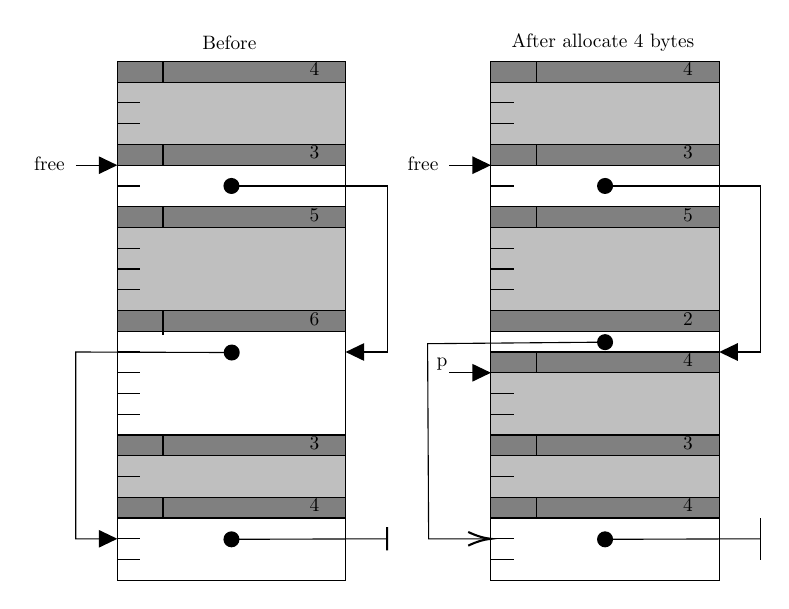
\begin{tikzpicture}[x=0.75pt,y=0.75pt,yscale=-1,xscale=1]
        \foreach \x in {20,60,90,140,200,230}{
            \draw  [fill=gray  ,fill opacity=1 ] (100,\x) -- (210,\x) -- (210,\x+10) -- (100,\x+10) -- cycle ;
        }
        
        \draw  [fill=lightgray  ,fill opacity=1 ] (100,30) -- (210,30) -- (210,60) -- (100,60) -- cycle ;
        \draw  [fill=white ,fill opacity=1 ] (100,70) -- (210,70) -- (210,90) -- (100,90) -- cycle ;
        \draw  [fill=lightgray ,fill opacity=1 ] (100,100) -- (210,100) -- (210,140) -- (100,140) -- cycle ;
        \draw  [fill=white  ,fill opacity=1 ] (100,150) -- (210,150) -- (210,200) -- (100,200) -- cycle ;
        \draw  [fill=lightgray  ,fill opacity=1 ] (100,210) -- (210,210) -- (210,230) -- (100,230) -- cycle ;
        \draw  [fill=white  ,fill opacity=1 ] (100,240) -- (210,240) -- (210,270) -- (100,270) -- cycle ;
        
        \foreach \x in {20,60,90,140,160,200,230}{
            \draw  [fill=gray  ,fill opacity=1 ] (280,\x) -- (390,\x) -- (390,\x+10) -- (280,\x+10) -- cycle ;
        }

        \draw  [fill=lightgray  ,fill opacity=1 ] (280,30) -- (390,30) -- (390,60) -- (280,60) -- cycle ;
        \draw  [fill=white  ,fill opacity=1 ] (280,70) -- (390,70) -- (390,90) -- (280,90) -- cycle ;
        \draw  [fill=lightgray  ,fill opacity=1 ] (280,100) -- (390,100) -- (390,140) -- (280,140) -- cycle ;
        \draw  [fill=white  ,fill opacity=1 ] (280,150) -- (390,150) -- (390,160) -- (280,160) -- cycle ;
        \draw  [fill=lightgray  ,fill opacity=1 ] (280,210) -- (390,210) -- (390,230) -- (280,230) -- cycle ;
        \draw  [fill=white  ,fill opacity=1 ] (280,240) -- (390,240) -- (390,270) -- (280,270) -- cycle ;
        \draw  [fill=lightgray ,fill opacity=1 ] (280,170) -- (390,170) -- (390,200) -- (280,200) -- cycle ;

        \foreach \x in {40,50,...,260}{
            \draw    (100,\x) -- (111,\x) ;
            \draw    (280,\x) -- (291,\x) ;
        }        
        
        \foreach \x in {20,60,90,160,200,230}{ \draw    (302,\x) -- (302,\x+10) ; }
        \foreach \x in {20,60,90,200,230}{ \draw    (122,\x) -- (122,\x+10) ; }
        
        \draw  (260,170) -- (278,170) ;
        \draw  (80,70) -- (98,70) ;
        \draw  (155,250.25) -- (230,250) ;
        \draw  (335,250.25) -- (410,250) ;
        \draw  (410,240) -- (410,260) ;        
        \draw  (260,70) -- (278,70) ;
        \draw  (122,140) -- (122,152) ;
        \draw  (155,80) -- (230,80) -- (230,160) -- (212,160) ;
        \draw  (335,155.25) -- (249.5,156) -- (250,250) -- (278,250) ;
        \draw  (335,80) -- (410,80) -- (410,160) -- (392,160) ;
        \draw  (155.13,160.25) -- (80,160) -- (80,250) -- (98,250) ;
        
        \draw [shift={(210,160)}, rotate = 360] [fill=black  ][line width=0.75]  [draw opacity=0] (8.93,-4.29) -- (0,0) -- (8.93,4.29) -- cycle;
        \draw [shift={(155,80)}, rotate = 0] [color=black  ][fill=black  ][line width=0.75] (0, 0) circle [x radius= 3.35, y radius= 3.35];
        \draw [shift={(100,250)}, rotate = 180] [fill=black  ][line width=0.75]  [draw opacity=0] (8.93,-4.29) -- (0,0) -- (8.93,4.29) -- cycle;
        \draw [shift={(155.13,160.25)}, rotate = 180.19] [color=black][fill=black ][line width=0.75](0, 0) circle [x radius= 3.35, y radius= 3.35];
        \draw [shift={(100,70)}, rotate = 180] [fill=black  ][line width=0.75]  [draw opacity=0] (8.93,-4.29) -- (0,0) -- (8.93,4.29) -- cycle;
        \draw [shift={(230,250)}, rotate = 539.81] [color=black  ][line width=0.75]    (0,5.59) -- (0,-5.59);
        \draw [shift={(155,250.25)}, rotate = 359.81] [color=black][fill=black ][line width=0.75] (0, 0) circle [x radius= 3.35, y radius= 3.35];
        \draw [shift={(390,160)}, rotate = 360] [fill=black ][line width=0.75]  [draw opacity=0] (8.93,-4.29) -- (0,0) -- (8.93,4.29) -- cycle;
        \draw [shift={(335,80)}, rotate = 0] [color=black ][fill=black ][line width=0.75] (0, 0) circle [x radius= 3.35, y radius= 3.35];
        \draw [shift={(280,70)}, rotate = 180] [fill=black ][line width=0.75]  [draw opacity=0] (8.93,-4.29) -- (0,0) -- (8.93,4.29) -- cycle;
        \draw [shift={(335,250.25)}, rotate = 359.81] [color=black][fill=black ][line width=0.75] (0, 0) circle [x radius= 3.35, y radius= 3.35];
        \draw [shift={(280,170)}, rotate = 180] [fill=black ][line width=0.75] [draw opacity=0] (8.93,-4.29) -- (0,0) -- (8.93,4.29) -- cycle;
        \draw [shift={(280,250)}, rotate = 180] [color=black ][line width=0.75] (10.93,-3.29) .. controls (6.95,-1.4) and (3.31,-0.3) .. (0,0) .. controls (3.31,0.3) and (6.95,1.4) .. (10.93,3.29);
        \draw [shift={(335,155.25)}, rotate = 179.5] [color=black ][fill=black ][line width=0.75] (0, 0) circle [x radius= 3.35, y radius= 3.35];
        
        \draw (67.33,69.33) node [scale=0.7] [align=left] {free};
        \draw (247.33,69.33) node [scale=0.7] [align=left] {free};
        \draw (256.5,166) node [scale=0.7] [align=left] {p};
        \draw (154,11) node [scale=0.7] [align=left] {Before};
        \draw (334,11) node [scale=0.7] [align=left] {After allocate 4 bytes};
        
        \foreach \x/\y in {24/4,64/3,94/5,144/6,204/3,234/4}{ \draw (195,\x) node [scale=0.7] [align=left] {\y}; }
        \foreach \x/\y in {24/4,64/3,94/5,144/2,164/4,204/3,234/4}{ \draw (375,\x) node [scale=0.7] [align=left] {\y}; }
    \end{tikzpicture}
    \caption{First-fit allocation policy}
    \label{fig:memman}
\end{figure}

If adjacent free blocks are available, the implementation combines them into a single larger block, minimizing the risk of fragmentation, making it suitable for applications that repeatedly allocate and free different sized blocks of RAM.

\begin{tcolorbox}
\ArrowBoldDownRight \textit{Note}: Because memory is statically declared, it will make the application appear to consume a lot of RAM, even before any memory has been allocated from it.
\end{tcolorbox}

\begin{tcolorbox}
\AsteriskBold \textit{Warning}: All the memory management APIs are NOT interrupt-safe. Use these APIs only from the base context.
\end{tcolorbox}

\begin{tcolorbox}
\AsteriskBold \textit{Warning}: The application is not exempt from memory leaks if the user does not perform adequate memory management. Here, the worst case scenario can occur in the absence of free memory. 
\end{tcolorbox}

\subsubsection{Memory pools}

A memory pool its a special resource that allows memory blocks to be dynamically allocated from a user-designated memory region. Instead of typical pools with fixed-size block allocation, the pools in QuarkTS can be of any size, thereby the user is responsible for selecting the appropriate memory pool to allocate data with the same size. 

The \textit{default} memory management unit resides in a memory pool object. Also called the \textit{default pool}. The total amount of available heap space in the default memory pool is set by \lstinline{Q_DEFAULT_HEAP_SIZE}, which is defined in \lstinline{qconfig.h}.

Besides the \textit{default} pool, any number of additional memory pools can be defined. Like any other object in QuarkTS, memory pools are referenced by handles, a variable of type \lstinline{qMemMang_Pool_t} \index{\lstinline{qMemMang_Pool_t}} and should be initialized before use with the \lstinline{qMemMang_Pool_Setup()} \index{\lstinline{qMemMang_Pool_Setup}} API function.
\medskip

\begin{lstlisting}[style=CStyle]
qBool_t qMemMang_Pool_Setup( qMemMang_Pool_t * const mPool, void* Area, 
                             size_t size )
\end{lstlisting}

\subsubsection*{Parameters}
\begin{itemize}
    \item \lstinline{mPool} : A pointer to the memory pool instance. 
    \item \lstinline{Area} :  A pointer to a memory region (\lstinline{qUINT8_t}) statically allocated to act as Heap of the memory pool. The size of this block should match the \lstinline{size} argument.
    \item \lstinline{size} : The size of the memory block pointed by \lstinline{Area}. 
\end{itemize}

To perform operations in another memory pool, besides the \textit{default} pool, an explicit switch should be performed using \lstinline{qMemMang_Pool_Select()} \index{\lstinline{qMemMang_Pool_Select}}. Here, a pointer to the target pool should be passed as input argument.  From now on, every call to \lstinline{qMalloc()}, or \lstinline{qFree()} will run over the newly selected memory pool. To return to  the \textit{default pool},  a new call to  \lstinline{qMemMang_Pool_Select()} is required passing \lstinline{NULL} as input argument. 
\medskip

\begin{lstlisting}[style=CStyle]
void qMemMang_Pool_Select( qMemMang_Pool_t * const mPool )
\end{lstlisting}

To keep track of the memory usage, the \lstinline{qMemMang_Get_FreeSize()} \index{\lstinline{qMemMang_Get_FreeSize}} API function returns the number of free bytes in the memory pool at the time the function is called.
\medskip

\begin{lstlisting}[style=CStyle]
size_t qMemMang_Get_FreeSize( void )
\end{lstlisting}

\subsubsection*{Usage example:}

\lstinputlisting[style=CStyle]{sec3memmangdem1.c}

\subsection{Trace and debugging}
QuarkTS include some basic macros to print out debugging messages. Messages can be simple text or the value of variables in specific base-formats. 
To use the trace macros, a single-char output function must be defined using the \lstinline{qTrace_Set_OutputFcn()} macro.\index{\lstinline{qTrace_Set_OutputFcn}}
\medskip

\begin{lstlisting}[style=CStyle]
qTrace_Set_OutputFcn( qPutChar_t fcn )
\end{lstlisting}

Where \lstinline{fcn} is a pointer to the single-char output function following the prototype:
\medskip

\begin{lstlisting}[style=CStyle]
void SingleChar_OutputFcn( void *sp, const char c ){
    /*
    TODO : print out the c variable using the
    selected peripheral.
    */
}
\end{lstlisting}

The body of this user-defined function should have a hardware-dependent code to print out the \lstinline{c} variable through a specific peripheral.

\subsubsection{Viewing variables}
For viewing or tracing a variable (up to 32-bit data) through debug, one of the following macros are available:
\index{\lstinline{qTrace_Var}} \index{\lstinline{qTrace_Variable}} \index{\lstinline{qDebug_Var}} \index{\lstinline{qDebug_Variable}}
\medskip

\begin{lstlisting}[style=CStyle]
qTrace_Var( Var, DISP_TYPE_MODE )
qTrace_Variable( Var, DISP_TYPE_MODE )
\end{lstlisting}
\begin{lstlisting}[style=CStyle]
qDebug_Var( Var, DISP_TYPE_MODE )
qDebug_Variable( Var, DISP_TYPE_MODE )
\end{lstlisting}

\subsubsection*{Parameters:}
\begin{itemize}
    \item \lstinline{Var} : The target variable. 
    \item \lstinline{DISP_TYPE_MODE } :  Visualization mode. It must be one of the following parameters(case sensitive): \lstinline{Bool}, \lstinline{Float}, \lstinline{Binary}, \lstinline{Octal}, \lstinline{Decimal}, \lstinline{Hexadecimal}, \lstinline{UnsignedBinary}, \lstinline{UnsignedOctal}, \lstinline{UnsignedDecimal}, \lstinline{UnsignedHexadecimal}. 
\end{itemize}

The only difference between \lstinline{qTrace_} and  \lstinline{Debug}, is that \lstinline{qTrace_} macros, print out additional information provided by the \lstinline{__FILE__}, \lstinline{__LINE__} and \lstinline{__func__} built-in preprocessing macros, mostly available in common C compilers. 

\subsubsection{Viewing a memory block}
For tracing memory from a specified target address, one of the following macros are available: \index{\lstinline{qTrace_Mem}} \index{\lstinline{qTrace_Memory}}

\begin{lstlisting}[style=CStyle]
qTrace_Mem( Pointer, BlockSize )
qTrace_Memory( Pointer, BlockSize )
\end{lstlisting}

\subsubsection*{Parameters:}
\begin{itemize}
    \item \lstinline{Pointer} : The target memory address.
    \item \lstinline{Size} : Number of bytes to be visualized.
\end{itemize}

Hexadecimal notation it's used to format the output of these macros.

\subsubsection{Usage}

In the example below, an UART output function is coded to act as the printer. Here, the target MCU is an ARM-Cortex M0 with the UART1 as the selected peripheral for this purpose.
\medskip

\begin{lstlisting}[style=CStyle]
void putUART1( void *sp, const char c ){
    /* hardware specific code */
    UART1_D = c;
    while ( !(UART1_S1 & UART_S1_TC_MASK) ) {} /*wait until TX is done*/ 
}
\end{lstlisting}  

As seen above, the function follows the required prototype. Later, in the main thread, a call to the \lstinline{qSetDebugFcn()} is used to set up the output-function.

\begin{lstlisting}[style=CStyle]
int main( void ){
   qTrace_Set_OutputFcn( putUART1 );
   ... 
   ...
}
\end{lstlisting}  

After that, trace macros will be available for use.

\begin{lstlisting}[style=CStyle]
void IO_TASK_Callback( qEvent_t e ){
   static qUINT32_t Counter = 0;
   float Sample;
   ...
   ... 
   qTrace_Message( "IO TASK running..." );
   Counter++;
   qTrace_Variable( Counter, UnsignedDecimal );
   Sample = SensorGetSample();
   qTrace_Variable( Sample, Float );
   ...
   ...
}
\end{lstlisting}